\documentclass[12pt]{article}
\usepackage{array}
\usepackage{amsmath}
\usepackage{mathtools}
\usepackage{gensymb}
\usepackage{graphicx}
\usepackage{float}
\usepackage{caption}
\usepackage{setspace}


\allowdisplaybreaks

\begin{document}

    \title{Coulomb's Law}
    \author{Ryan Coyne, Ben Eid, Erin Snook}
    \maketitle
    \section{Abstract}
        We used charged balls hanging from strings to measure how the force, \(F_E\), between two charged bodies changes with the distance between them, \(r\). We found that \(F_E \propto r^{-(2.36 \pm 0.28)}\). We also found that the charges on each ball in the respective trials were \(\pm 0.14\) nC, \(\pm 1.9\) nC, \(\pm 1.1\) nC, and \(\pm 0.10\) nC. From these charges, we found that the difference between the number of protons and electrons within the balls in each trial was approximately \(8.8 \times 10^8\), \(1.2 \times 10^9\), \(6.9\times 10^9\), and \(6.2\times 10^8\) respectively.

    \section{Introduction}
        When two point charges have the same type of electric charge, either positive or negative, they repel each other. The magnitude of this repulsion is dependent in some way on the distance between them and the charge of each. This relationship between the force between charges is called Coulomb's law and is typically written as 
        \begin{equation}
            F_E = k\frac{|q_1q_2|}{r^2}.
        \end{equation}
        Where \(q_1\) and \(q_2\) are the charges and \(k=8.99\times 10^9\) \(\mathrm{Nm^2/C^2}\) is Coulomb's constant.  The vacuum permittivity constant, \(\epsilon_0=8.85\times 10^{-12}\ \mathrm{C^2/Nm^2}\), can be used instead of \(k\) with the relation
        \begin{equation}
            k = \frac{1}{4\pi \epsilon_0}.
        \end{equation} 

        Coulomb's law says that the electric force is proportional to \(1/r^2\). Therefore, the force between two weakly charged bodies should decrease quickly but measurably as they move apart.
    \section{Procedure}
        Begin by suspending a metal rod horizontally above a table. Make 8 marks on the rod that are approximately 1 cm apart and record the distance between each. Hang two pith balls from the rod using string, one at the first mark and the other at the second. Measure the distance from the top of the string to the center of the balls and adjust so that it is equal for each ball. Rub a plastic rod with wool and use it to charge the balls. Measure and record the distance between each ball. Move the second ball to each mark made on the rod and record the distance between the balls. Touch the balls to discharge them. Repeat the experiment three more times. 
        \begin{figure}[H]
            \centering
            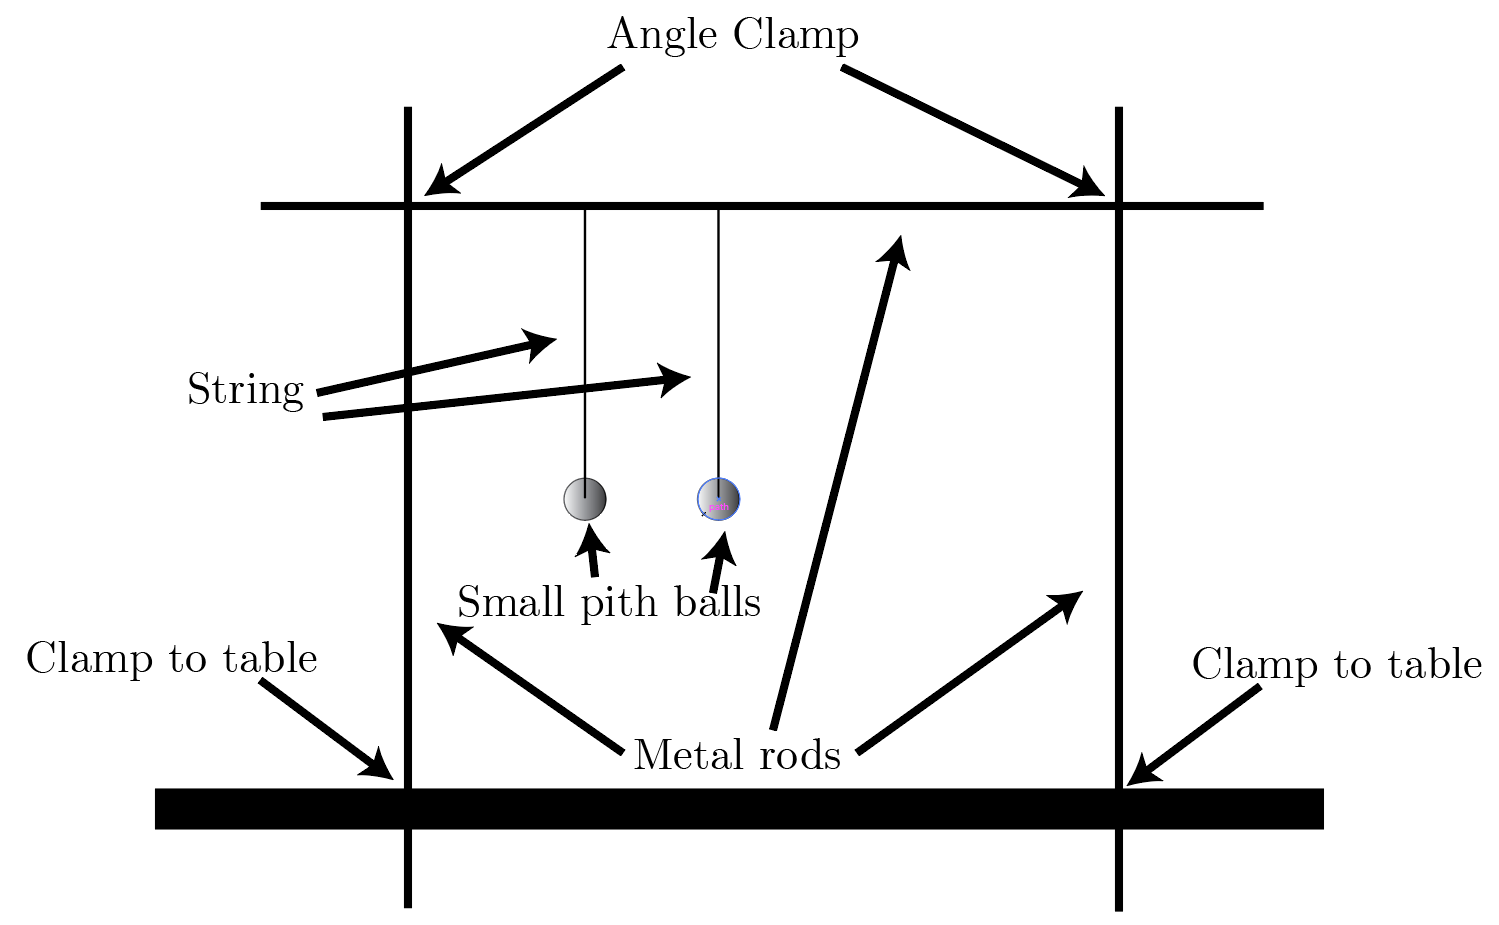
\includegraphics[width=0.9\linewidth]{experimental_setup.png}
        \end{figure}
    \section{Data}
        \begin{table}[H]
            \centering
            \begin{tabular}{c|c|c}
                &\(r\) (m)& \(w\) (m)\\
                \hline
                1&0.0326&	0.0105\\
                &0.0398&	0.0191\\
                &0.0436&	0.0275\\
                &0.0465&	0.0368\\
                &0.0557&	0.0467\\
                &0.0586&	0.0562\\
                &0.0673&	0.0648\\
                \hline
                2&0.0672&	0.0648\\
                &0.0612&	0.0562\\
                &0.0524&	0.0467\\
                &0.0456&	0.0368\\
                &0.0373&	0.0275\\
                &0.0302&	0.0191\\
                &0.0254&	0.0105\\
                \hline
                3&0.068&	0.0648\\
                &0.061&	0.0562\\
                &0.053&	0.0467\\
                &0.045&	0.0368\\
                &0.038&	0.0275\\
                &0.032&	0.0191\\
                &0.031&	0.0105\\
                \hline
                4&0.026&	0.0105\\
                &0.034&	0.0191\\
                &0.039&	0.0275\\
                &0.043&	0.0368\\
                &0.048&	0.0467\\
                &0.066&	0.0648\\
            \end{tabular}\\
            \caption{Measured values of \(r\) and \(w\).}
        \end{table}
        \begin{table}[H]
            \centering
            \begin{tabular}{c|c}
                \(l\) (m) & \(m\) (g)\\
                \hline
                0.2365 & 0.030\\
                0.2383 &\\
                0.2354 &\\
                0.2384 &\\
            \end{tabular}
            \caption{Measured values of \(l\) and \(w\).}
        \end{table}
        \begin{figure}[H]
            \centering
            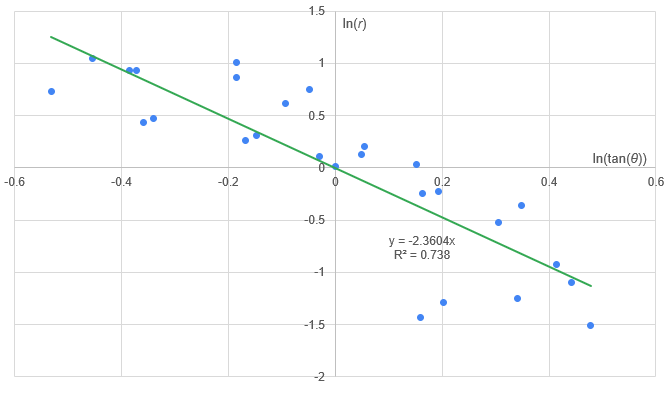
\includegraphics[width = \linewidth]{linest.png}
            \caption{Plot of \(\ln \tan \theta\) vs \(\ln r\) with fit to determine \(\overline{n} \pm \sigma_n\)}
        \end{figure}
    \section{Calculations}
        \begin{figure}[H]
            \centering
            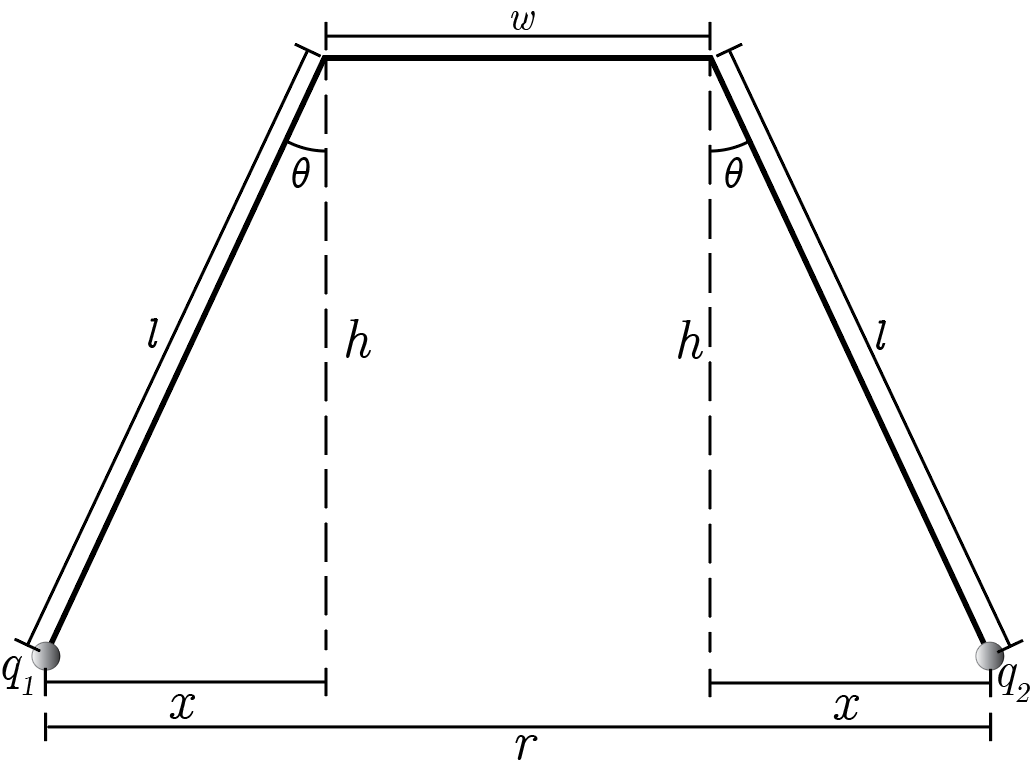
\includegraphics[width=0.75\linewidth]{diagram.png}
        \end{figure}
        \begin{figure}[H]
            \centering
            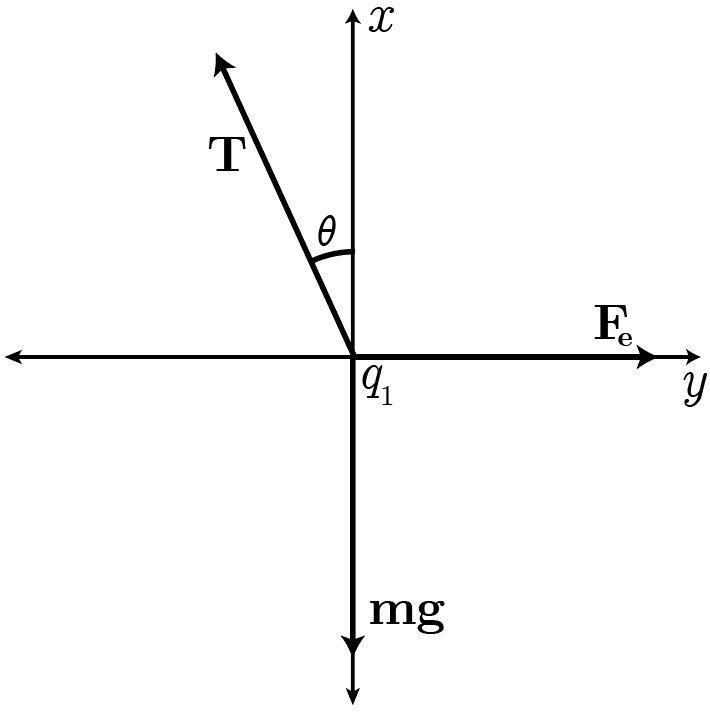
\includegraphics[width=0.7\linewidth]{freebody.png}
        \end{figure}
        \begin{alignat*}{3}
            (1)~~
            &F_E = \frac{|q_1q_2|}{4\pi \epsilon_0 r^n}\\
            &\Sigma \mathbf{F} = m\mathbf{a} = 0\\
            &x: -T\sin(\theta) + F_E = 0\\
            &y: T\cos(\theta) - m\mathbf{g} = 0\\
            &\tan(\theta) = \frac{\mathbf{F}_E}{m\mathbf{g}}\\
            &\qquad\quad\;\!\! = \frac{|q_1q_2|}{4\pi \epsilon_0 r^nm\mathbf{g}}\\
            &\text{Let}\ a = \frac{|q_1q_2|}{4\pi \epsilon_0 m\mathbf{g}}\\
            &\tan(\theta) = \frac{a}{r^n}\\
            &\ln(\tan(\theta)) = \ln(a) - n\ln(r)\\            
        \end{alignat*}
        \begin{alignat*}{3}
            (2)\ \ 
            &\tan(\theta) = \frac{x}{h}\\
            & l^2 = x^2 + h^2\\
            & h = \sqrt{l^2-x^2}\\
            &\tan(\theta)= \frac{x}{\sqrt{l^2-x^2}}\\
            &r = w+2x\\
            &x = \frac{r-w}{2}\\
            &\tan(\theta) = \frac{\frac{r-w}{2}}{\sqrt{l^2 - (\frac{r-w}{2})^2}}
        \end{alignat*}
        \begin{alignat*}{3}
            (3)~~
            &&a &=\frac{|q_1q_2|}{4\pi \epsilon_0 m\mathbf{g}}\\
            && q_1 &= q_2 = q\\
            &&\ln a &= -3.39\\
            && e^{-3.39} &= \frac{q^2}{4\pi \epsilon_0 m\mathbf{g}}\\
            && q &= \sqrt{e^{-3.39}\cdot4 \pi \epsilon_0 m\mathbf{g}}\\
            &&& = 0.14 \text{ nC}\\
            &&e &= 1.60217663\times 10^{-19} \text{ C}\\
            &&\frac{q}{e} &=8.8 \times 10^8
        \end{alignat*}
        \begin{alignat*}{3}
            (4)~~
            &&F_E &= \frac{(0.14 \text{ nC})^2}{4\pi\epsilon_0 \cdot (0.0326\ \text{m})^2}\\
            &&&= 0.0000165832 N\\
            &&F_G &= 0.000030 \text{ kg} * 9.8\ \mathrm{m/s^2}\\
            &&& = 0.000294\text{ N}\\
            &&\frac{F_E}{F_G} &= 0.056
        \end{alignat*}
    \section{Conclusion}
        The exponent of \(r\) in Coulomb's law, \(n\), was measured to be \(2.36 \pm 0.28\). This is a reasonably good measurement because it is well within two standard deviations of the expected value, 2. We performed the experiment 6 times but discarded two of the data sets because some measurements of \(r\) on those sets were less than the measured value of \(w\). These were clearly inaccurate and resulted in undefined values for \(\ln\tan\theta\), rendering the calculations impossible. The measurements of \(r\) were difficult to take because the balls were swinging, but it's possible the errors could have been avoided by taking the measurements more carefully.
\end{document}